\chapter{Searching for PBH Candidates in \Fermi-LAT 3FGL Catalog}\label{chapter:pbh_analysis}


\Fermi-LAT surveys the entire sky approximately every three hours, and has relatively uniform exposure over long time scales; in our dataset of 4 years, the exposure above 1 GeV varies by approximately 40\% over the entire sky. Combined with a large effective area (approximately 1 m$^2$ between 1 GeV and 1 TeV), this makes it an ideal instrument for detecting a large number of gamma-ray point sources. 
The most complete catalog of point sources is currently the third \Fermi point source catalog \citep[3FGL, ][]{2015ApJS..218...23A} (see Section \ref{sec:analysisTools} for a brief description of the methodology that the \Fermi-LAT collaboration uses to build catalogs). 
The 3FGL contains sources that are significantly detected above 100 MeV and spans the first 4 years of the \Fermi mission. 
%A complete description of the 3FGL can be found in \citep{2015ApJS..218...23A}. .
In this chapter, I use the 3FGL catalog to search for PBH candidates and to constrain the local PBH evaporation rate.

\section{Search Strategy}
\label{sec:search}
The first step in selecting PBH candidates in the 3FGL catalog was excluding from further consideration point sources associated with known astrophysical sources (such as blazars). Of 3033 sources in the 3FGL catalog, 1010 are unassociated sources. Also excluded were a further 468 unassociated sources that lie within $10^\circ$ of the Galactic plane. The analysis was restricted to high-latitude sources for three reasons: (a) detectable PBHs are expected be distributed isotropically given the detectability distances estimated in Section \ref{sec:sens}, while astrophysical sources are concentrated along the Galactic plane, (b) association of extragalactic sources such as blazars is easier at high latitude 
\citep[see, e.g.][]{2015ApJ...810...14A}, and (c) the reduced Galactic diffuse emission at high latitude makes proper motion identification easier.

The spectra of the remaining unassociated 3FGL sources were next compared with the time-integrated PBH gamma-ray spectrum.
Spectra of the candidate sources are reported in the 3FGL as fluxes in 5 energy bands (0.1 -- 0.3, 0.3 -- 1, 1 -- 3, 3 -- 10, and 10 -- 100 GeV).
The time-integrated PBH spectrum depends on two parameters: initial mass (or temperature), and the distance to the Earth (equivalent to an overall normalization).
These two parameters were varied to obtain the best fit to the candidate source spectra in the five energy bands.
The quality of the fit to the 3FGL spectrum was determined by calculating the value of the $\chi ^2$ over the five energy bands:

\noindent
\begin{equation}
\chi^2 = \sum_{i = 1}^{5} \frac{(\Phi_i-\Psi_i )^2}{\sigma_i^2}, 
\end{equation}
where $\Phi_i$ is the PBH spectrum integrated over the width of bin $i$ and $\Psi_i$ is the flux in bin $i$ reported in the 3FGL. Here $\sigma_i$ represents the uncertainty on the flux in bin $i$.
In the 3FGL, flux uncertainty is represented by a 68\% confidence interval; the value of the uncertainty can then be written as the difference between the best-fit flux and either the upper or lower bound.
We set $\sigma_i$ to be the larger of the two in order to be conservative.
We require the value of the best-fit $\chi^2$ to be below the critical value of 11.3, which corresponds to 99\% exclusion for 5 degrees of freedom and 2 parameters. In other words, sources with a $\chi ^2$ value greater than 11.3 have only a 1\% chance of being spectrally consistent with a PBH. After the spectral consistency was computed, 318 sources out of the 542 unassociated candidates remained as plausible PBH candidates.
The candidate sources next underwent a check for proper motion. 

\subsection{Proper Motion}\label{sec:propmotion}
Several algorithms were examined for the ability to discriminate between moving and stationary sources.
Inspired by the track reconstruction algorithms used in the \Fermi-LAT tracker, the first algorithm studied was a Kalman filter, implemented with a model of a moving source (with Gaussian uncertainty at each data point). 
The Kalman filter was successful was successful in Monte Carlo simulations of reconstructing the velocity of a moving point source, but is not easily adapted to cases where the signal is subdominant to background.

Next studied was an algorithm which computed the moment of inertia tensor of the source photon locations.
Subsequent diagonalization of the moment of inertia tensor gave the spatial eigenvectors and eigenvalues associated with the source; any motion was assumed to take place along the larger of the two eigenvectors.
The photons were divided into two groups according to which side of the center of mass (along the eigenvector) they fell, and the mean arrival times of the two groups of photons were compared.
However, the moment of inertia depends on the square of the distance of each photon from the center of mass.
Therefore the algorithm was found to be too sensitive to the diffuse background, which is distributed isotropically across the region of interest, and nearby non-candidate point sources.

After further testing, an algorithm was built which uses the method of maximum likelihood estimation to (a) weight background photons given a model of the ROI, and (b) reconstruct the proper motion of the candidate source.
The algorithm works as follows:
\begin{enumerate}
\item
All source-class photons above 1 GeV within $5^\circ$ of the source's reported 3FGL location were collected.
The time range (August 2008 to July 2012) and data reconstruction (\texttt{P7REP\char`_SOURCE\char`_V15}) were consistent with that of the data used to construct the 3FGL.
Since the angular resolution of the \Fermi LAT decreases quickly below 1 GeV, including photons below 1 GeV did not have a significant impact on the final results.
\item 
Data covering a longer time range (August 2008 to July 2017) and a more recent event reconstruction (\texttt{P8R2\char`_SOURCE\char`_V6}) were held in reserve for validation, and was used to test the PBH hypothesis for any sources that passed the proper motion cut.

\item
The expected number of photons $N$ from the source of interest was calculated by multiplying the flux in each energy bin by 
the \Fermi-LAT exposure at the bin's midpoint energy, and summing over the three relevant bins (1 -- 3 GeV, 3 -- 10 GeV, 10 -- 100 GeV). 
\item 
\label{step:prop_motion_likelihood}
In order to estimate the velocity of a PS, the maxima of the likelihood function $\mathcal{L}(\vec{x_i},t_i,\vec{x_0},\vec{v_0})$ are compared in two cases: 
fixed $\vec{v_0}=0$ and free $\vec{v_0}$. 
The point spread function of \Fermi-LAT was approximated as a Gaussian for simplicity.
The likelihood function is given by multiplying over $N$ photons around the initial position of the source:

\noindent
\begin{equation}
\label{eq:vlike}
\mathcal{L} = \prod_{i=1}^{N}w_i\times \textup{exp} \big\{\frac{{-(\vec{x_i}-\vec{x_0}-\vec{v_0}t_i)^2}}{{\sigma_i^2}}\big\}
\end{equation}
where $\vec{x_i}$ is the coordinates of the photon, $\vec{v_0}$ is the proper motion of the source, $t_i$ is the photon arrival time, $\vec{x_0}$ is the source location at the beginning of the observation time, and $\sigma_i$ is the 68\% angular containment radius for a photon at energy $E_i$, which is $\sim 0.7^\circ$ at 1 GeV \citep{2013arXiv1304.5456B}.
Here $w_i$ is a weight assigned to each photon, the calculation of which is defined in Section \ref{sec:likelihood}. 

In practice, the natural logarithm of the likelihood is used:
\begin{equation}
\label{eq:vloglike}
\log \mathcal{L} = \sum_{i=1}^{N}\log w_i-\frac{{(\vec{x_i}-\vec{x_0}-\vec{v_0}t_i)^2}}{{\sigma_i^2}}
\end{equation}

The main difficulty is separating the $N$ photons attributed to the source from background photons.
The algorithm chooses a 4-dimensional grid of points around an initial value of $\vec{x_0}$ and $\vec{v_0} = 0$, and for each grid point finds the $N$ photons
inside the $5^\circ$ ROI that have the highest contribution to $\log \mathcal{L}$, i.e. the photons which most likely belong to the source given a particular position and velocity.
Therefore the weights $w_i$ do not appear as a prefactor in Eqs \ref{eq:vlike} and \ref{eq:vloglike} because the $N$ best-fit photons change given different assumptions of $\vec{x_0}$ and $\vec{v_0}$.
The best-fit $\vec{x_0}$ and $\vec{v_0}$ are found by maximizing $\Delta \log \mathcal{L} = \log \mathcal{L} - \log \mathcal{L}(\vec{v_0}=0)$ on the grid.
With the additional degrees of freedom from allowing $\vec{v_0}$ to float, the value of $\Delta \log \mathcal{L}$ is always nonnegative. 

MC simulations (described in Section \ref{sec:MClimit}) demonstrate that this algorithm tends to underestimate the input velocity by $\approx 25\%$;
the best-fit velocity should therefore be considered a lower bound on the true velocity and sufficient for our purpose of separation of moving and stationary sources.
The underestimation occurs because source photons that are far away from the average source position have lower weights and so are less often included in the likelihood calculation.
In their place are background photons, whose distribution in time is random, and therefore cause the algorithm to favor a slower overall velocity.
%The $N$ photons used in the calculation will generally change over the course of the maximization procedure, because it is not possible to discriminate between individual source and nearby background photons. However, the algorithm converges if the source is sufficiently brighter than the background. 
\item 
The significance of $\Delta \log \mathcal{L}$ for each source was found by assigning random times $t_i$ drawn from a flat distribution to each photon but fixing the positions $\vec{x_i}$ of all the photons, and reoptimizing $\Delta \log \mathcal{L}$. 
This process was repeated 50 times for each source, and the original value of $\Delta \log \mathcal{L}$ was compared with the distribution of $\Delta \log \mathcal{L}$ for the data sets scrambled in time to find a local significance $\sigma$:

\noindent
\begin{equation}
\sigma = \frac{\Delta \log \mathcal{L}_0 - \overline{\Delta \log \mathcal{L}_s}}{\textup{std}(\Delta \log \mathcal{L}_s)},
\end{equation}
where $\Delta \log \mathcal{L}_0$ is the original value of the improvement in likelihood, $\overline{\Delta \log \mathcal{L}_s}$ is the mean of the scrambled likelihood improvements, and $\textup{std}(\Delta \log \mathcal{L}_s)$ is the standard deviation of the scrambled likelihood improvements.
\item
A cut on the local significance for each source was made at $3.6 \sigma$ which corresponds to a global significance of $2 \sigma$ for 318 sources. 
\end{enumerate}

The key step in this process is the maximization of likelihood in Step \ref{step:prop_motion_likelihood}. 
Because the algorithm only considers the $N$ best photons at each grid point, it is highly resistant to background photons in cases where the source is undergoing proper motion; background photons are generally distributed evenly across time which means they are unlikely to fit well to the reconstructed path of the source at the grid point under consideration.
Monte Carlo simulations of PBHs show that the algorithm is highly successful (See Figure X) at reconstructing the true velocity in cases where the PBH has a lifetime at least as long as the time considered.
In cases where the PBH evaporates before the end of the time period, the velocity reconstruction is not accurate, but the discrimination between moving and stationary sources is still sufficient.
Long-lived PBHs far outnumber short-lived ones due to the nonlinear nature of the evaporation process- see Equation \ref{eq:Tdistr}- so the algorithm was designed to maximize sensitivity to long-lived PBHs.

\begin{figure}
\begin{center}
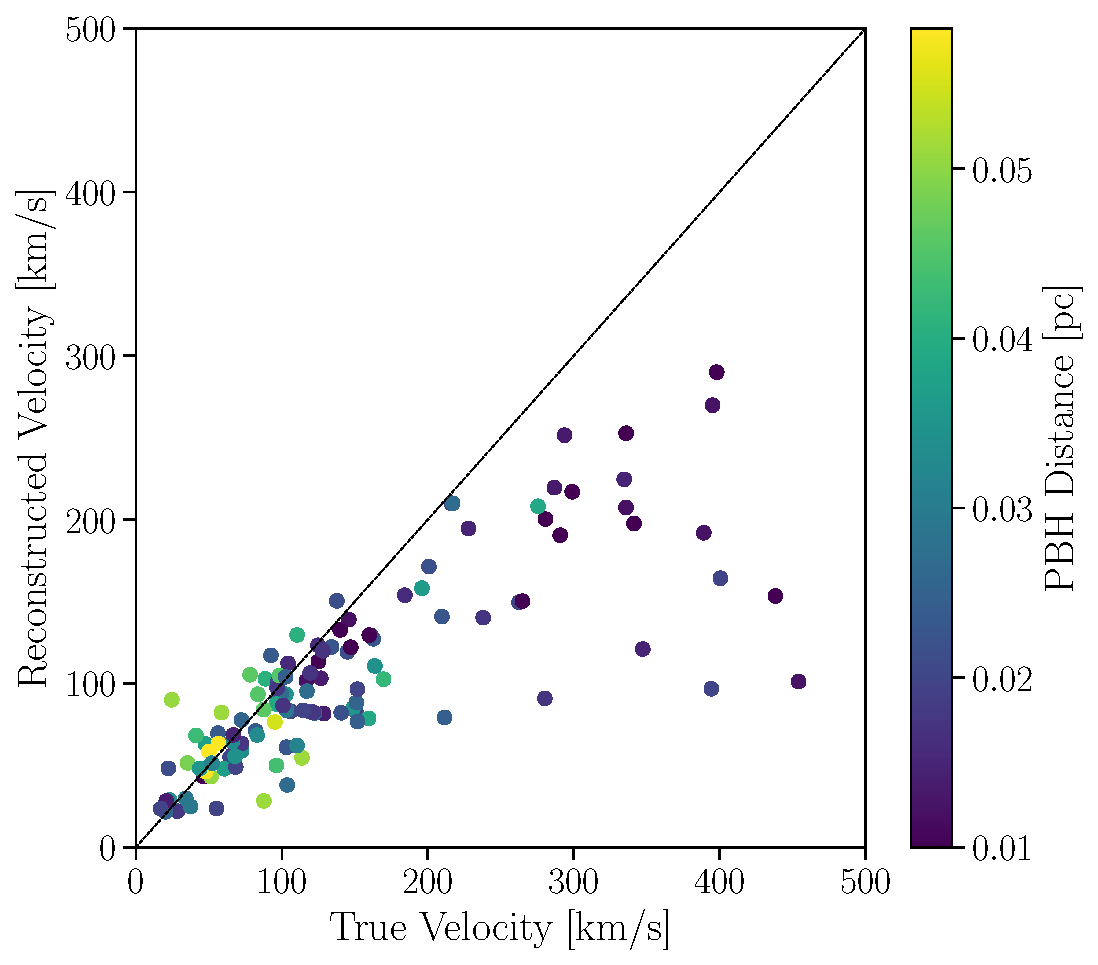
\includegraphics[width=0.9\columnwidth]{figures/reconstructedVelocity.pdf}
\caption{
\label{fig:reconstruction}
Reconstructed velocities from MC simulations (described in Section \ref{sec:MClimit}). The reconstruction is not perfect due to the presence of background photons and statistical fluctuations, and works best for slow-moving sources. At high velocities, the reconstructed velocity is generally below the true velocity because of the photon weighting scheme (Section \ref{sec:likelihood}) which favors slow-moving sources. The coloring indicates distance, showing that distant sources must be moving relatively slowly to pass the selection criteria.
}
\end{center}
\end{figure}

A single source (3FGL J2310.1$-$0557, see Section \ref{sec:j2310} for a discussion of this source) exceeded this cut on local significance, and the standard deviation of the local significances of the entire set of candidates was 1.03, which is consistent with statistical fluctuations.
After examining the data held in reserve for J2310.1$-$0557 (described in Section \ref{sec:j2310}), it was concluded that no likely PBH candidates exist in the 3FGL catalog.

\subsection{Photon Weights}
\label{sec:likelihood}

The photon weights $w_i$ in equations \ref{eq:vlike} and \ref{eq:vloglike} are defined as the probability that a given photon originated from the candidate PS, and are calculated by performing a standard likelihood optimization with the \Fermi Science Tool {\tt gtlike}\footnote{Science Tools version v10r0p5, available at \url{http://fermi.gsfc.nasa.gov/ssc/data/analysis/software}}.
The model used includes all 3FGL PS within 5$^\circ$ of the candidate source, as well as the standard Pass 7 models for Galactic and isotropic diffuse emission.
The candidate source is modeled as an extended source with a radial Gaussian profile with $\sigma=0.25^\circ$ instead of a PS, in order to account for the possibility of small amounts of proper motion.
The data were binned into three logarithmically spaced energy bands between 1 GeV and 100 GeV and in $0.1^\circ \times 0.1^\circ$ spatial pixels.
After the model was optimized by {\tt gtlike}, weights were assigned to each photon (described its coordinates $x$, $y$, and energy $E$) by calculating the fraction of the flux belonging to the candidate source in each pixel:

\begin{equation}
w_{x,y,E} = \frac{\Phi'(x,y,E)}{\sum_i \Phi_i(x,y,E)}
\end{equation}
where $\Phi'(x,y,E)$ is the predicted flux from the candidate source in the pixel and $\Phi_i(x,y,E)$ are the fluxes from all the sources in the model.

In addition, the 3FGL PS were masked by assigning a weight of zero to all the photons which fell in a pixel more than 1$^\circ$ from the candidate source position where the summed contribution of the non-candidate PS fluxes exceeded 10\% of the total flux in that pixel.
This meant that all the photons in the calculation had a high probability of originating only from either the candidate source or the diffuse background.

The weighting has little impact on the reconstruction of proper motion because individual photon weights do not change as the likelihood maximization from step \ref{step:prop_motion_likelihood} optimizes $\vec{x_0}$ and $\vec{v_0}$.
However, weighting the photons in this way prevents the algorithm from interpreting photons from nearby sources as originating from the candidate source.
Without weighting, nearby flaring sources could mimic a moving source and therefore lead to false positives.

The radial Gaussian weighting of the candidate PS does reduce the accuracy of reconstructing the proper motion of fast-moving sources- see Figre X.
Because the main purpose of the algorithm is simply to discriminate between moving and non-moving sources, this was deemed an acceptable tradeoff for the improvement in background rejection that comes from the weighting.

\subsection{J2310.1$-$0557}
\label{sec:j2310}
The source J2310.1$-$0557 passed the proper motion cut with a significance of 4.2$\sigma$, and was therefore investigated further.
Approximately 9 years (August 2008 to July 2017) of Pass 8 (\texttt{P8\char`_SOURCE\char`_V6}) data above 1 GeV in an ROI of 5$^\circ$ around the source location were collected.
The increased statistics and improved angular resolution of the Pass 8 data set clearly indicated that J2310.1$-$0557 lies approximately 1$^\circ$ away from a separate, highly variable source of gamma rays which is not in the 3FGL catalog.
This source flared brightly (approximately 150 photons above 1 GeV) on 7 March 2011 (near the end of the 3FGL time period) but was quiet for the remainder of the period.
We found that the position of the source was consistent with the Sun, which flared brightly on the same date \citep{2011ATel.3214....1A}.
$\gamma$-ray emission from the Sun and Moon was not included in the models of the ROI.

The effect of the solar flare near a candidate PBH was to mimic a moving source, which explains why the proper motion algorithm returned a positive result. 
Because the sources in the Monte Carlo simulation described in Section \ref{sec:MClimit} are placed at random points on the sky, similar false positives are expected to occur in the simulations.
Therefore,the upper limit on PBH evaporation rate is reported as if one source passed our criteria, even though J2310.1$-$0557 is not a good PBH candidate.
Incidentally after the publication of the 3FGL source list, J2310.1$-$0557 was found to be a millisecond pulsar\footnote{See https://confluence.slac.stanford.edu/display/SCIGRPS/LAT+Pulsations+from+PSR+J2310-0555}.

\begin{figure}
\begin{center}
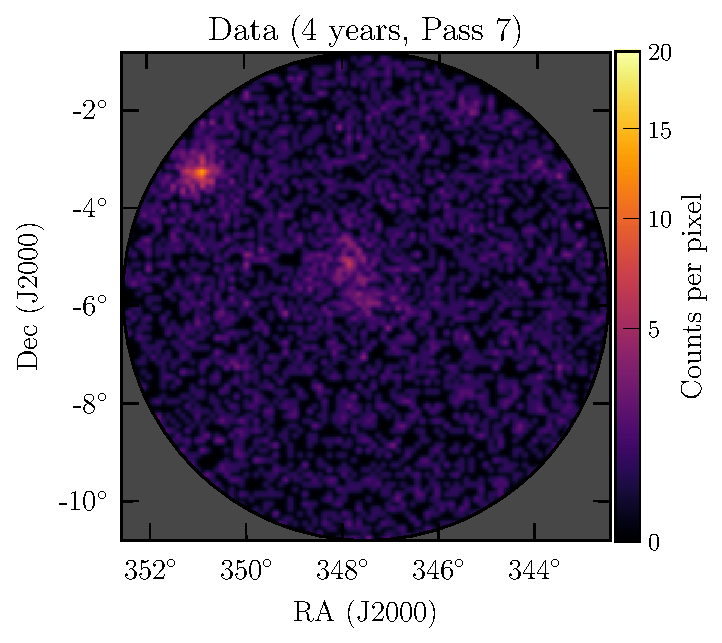
\includegraphics[width=0.45\columnwidth]{figures/3fgl_overlay.pdf}
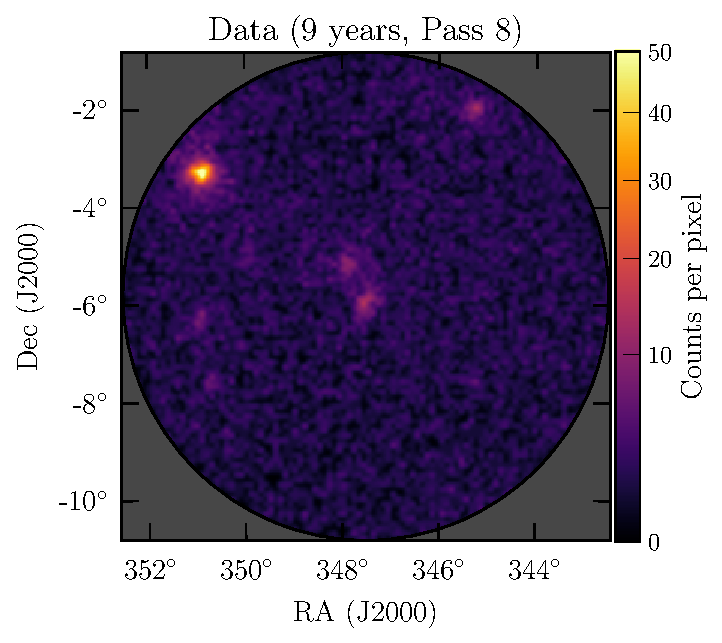
\includegraphics[width=0.45\columnwidth]{figures/4fgl_overlay.pdf}
\caption{
\label{fig:j2310}
{\it Left Panel:} 5$^\circ$ ROI around 3FGL J2310.1$-$0557, using the 4 years of data from the 3FGL analysis. The source at the center of the image appears to be extended due to the 7 March 2011 solar flare just to the upper-left of the candidate source.
{\it Right Panel:} The same ROI using 9 years of data and using the more recent Pass 8 reconstruction algorithms. The formerly extended source is clearly resolved as two separate sources.
}
\end{center}
\end{figure}
\section{Limits on PBH\MakeLowercase{s}}
\label{sec:MClimit}

An analytic derivation of the upper limit on the local PBH evaporation rate is difficult due to the complex nature of the variables in question.
For a PBH to pass all the cuts in Section \ref{sec:search}, it must have three main characteristics: (a) be listed as a PS in the 3FGL, (b) have a reconstructed spectrum which is consistent with a PBH, and (c) yield a significant proper motion when analyzed with the algorithm described in Section \ref{sec:propmotion}.
Each step in this process depends intimately on models of the background, as well as the temperature, distance, and velocity of the PBH.
Therefore, the efficiency for detecting PBHs was derived from Monte Carlo (MC) simulations.
Upper limits on the local PBH evaporation rate were then placed using the derived efficiency.

A sample of PBHs was generated within 0.08 pc of the Earth with uniform spatial density.
The PBH velocites were randomly sampled from a Gaussian distribution that had an average value of $250\rm\,km\, s^{-1}$, which is close to an upper bound on orbital velocity of the Sun around the Galactic center \citep{1999MNRAS.310..645W, 2008ApJ...684.1143X, 2009PASJ...61..227S, 2010ApJ...720L.108G, 2010MNRAS.402..934M, 2011MNRAS.414.2446M},
and dispersion equal to the local velocity dispersion of dark matter, $270\rm\,km\, s^{-1}$ \citep{2010JCAP...02..030K}.
At the end of this section, different assumptions about the PBH distribution (such as the relative velocity and velocity dispersion) are used to calculate an upper limit for the evaporation rate, providing an estimate of the systematic uncertainty.

The PBH population is assumed to have a constant rate of PBH evaporations, $\dot{\rho}_{\rm PBH} = const$ which is reasonable given the short time period of the search (4 years) compared with the age of the Universe.
A constant rate of evaporation implies that the derivative of the PBH density is related to the PBH temperature as:

\noindent
\begin{equation}
\label{eq:Tdistr}
\frac{d \rho_{\rm PBH}}{d T} \propto T^{-4}.
\end{equation}

This relation can be derived as follows: Let $\rho_{\rm PBH}(T)$ be the density of PBHs with temperature larger than $T$. If $\tau(T)$ is the lifetime of a PBH with temperature $T$, then all PBHs with $T' > T$ will evaporate during time $\tau$. Consequently,

\noindent
\begin{equation}
\label{eq:rho0}
\rho_{\rm PBH}(T) = \int_0^{\tau(T)} \dot{\rho}_{\rm PBH} dt = \dot{\rho}_{\rm PBH}\; \tau(T).
\end{equation}
Now taking into account that $\tau \propto T^{-3}$ and differentiating with respect to $T$ to get
Equation (\ref{eq:Tdistr}).

The following steps were performed in the derivation of the PBH evaporation rate limit:
\vspace{-2mm}
\begin{enumerate}
\item
\label{item:make_pbhs}
A sample of PBHs $(T_i, \vec{x}_i, \vec{v}_i)$ was simulated with temperatures $T_i>5\: {\rm GeV}$ and $T_i<60\: {\rm GeV}$ distributed according to Equation (\ref{eq:Tdistr}), and distances $R_i$ within $R < 0.08$ pc around the Earth. 
The velocities $v_i$ of the sample PBHs were distributed with mean equal to the orbital velocity of the Sun, 
$v_{\rm rot} = 250\; {\rm km\: s^{-1}}$,
and dispersion $v_{\rm disp} = 270\; {\rm km\: s^{-1}}$.
\item
The photons emitted by each PBH were simulated over the 4 year 3FGL time period, consistent with the parent PBH evolution.
A time step of $\Delta t = 1$ day was used in modeling the evolution of the PBH position and temperature since \Fermi LAT has relatively uniform exposure on time periods longer than 1 day; because the analysis takes place over 4 years the uneven exposure on timescales shorter than 1 day are negligible.
 The number of photons detected by the \Fermi LAT each day was given by a Poisson random value with a mean of 

\noindent
\begin{equation}
\overline{N(t)} = \frac{ \Delta t}{4\pi R^2}\int_{\textup{E=100 MeV}}^{\textup{E=500 GeV}} {\Phi(E,t)} A(E) dE,
\end{equation}
where $A$ is defined as the average \Fermi-LAT exposure per unit time at the position of the simulated PBH, and $R$ is the distance from the Earth.
The energy of each photon was found by random sampling of $\Phi(E,t)\times A(E)$. 
PBH emission spectra $\Phi(E,t)$ are discussed in Appendix \ref{chapter:pbh_spectrum}. 
The positions of the photons were randomized according to the \Fermi-LAT point-spread function (modeled as a Gaussian distribution) at the photon energy.

\item
\label{item:detection}
The list of simulated PBH photons was concatenated to the real photons present within $5^\circ$ of the final location of the PBH, with the same data selection as the 3FGL. A likelihood fit using the \Fermi Science Tool {\tt gtlike} was performed in a $7^{\circ}\times7^{\circ}$ ROI centered at the same location, using a model of the sky which included all 3FGL sources within $5^\circ$ of the ROI center, as well as models of the isotropic diffuse and Galactic diffuse emission\footnote{The models used were the standard Pass 7 (for consistency with the 3FGL) diffuse emission models available from \url{https://fermi.gsfc.nasa.gov/ssc/data/access/lat/BackgroundModels.html}}. The PBH was modeled as a source with a LogParabola spectrum, with fitting parameters restricted to the ranges $1.2<\alpha<3.0$ and $0.0<\beta<1.0$. Once the likelihood maximization was complete, the PBH was considered detected if its TS value was greater than 25, which is consistent with the 3FGL cutoff.
\item
\label{item:spectrum}
If the PBH source was detected, the results from the likelihood fit were used to find the source flux in the five energy bins reported in the 3FGL catalog. The spectral consistency with a PBH spectrum was then calculated in the same way as described in Section \ref{sec:search}.
\item 
\label{item:motion}
If the source was found to be spectrally consistent with a PBH, the significance of any proper motion was evaluated by the algorithm described in Section \ref{sec:search}. The combined efficiency of steps \ref{item:detection}$-$\ref{item:motion} is displayed in Figure \ref{fig:det_map}. We smoothed the results by convolving the detectability map with a 3$\times$3 matrix of ones, which had a minor ($\approx$ 8\%) impact on the resulting limit. The impact of fluctuations was quantified by observing the change in the limit as the number of simulations increased; we found that an increase of the number of simulations by 100\% had less than a 20\% change in the resulting limit.
\item 

\label{step:eff}
To derive an upper limit on the number of PBH evaporations in our search region, we begin with the number of expected detections:

\noindent
\begin{equation}
\label{eq:N_det}
N = \rho \epsilon V,
\end{equation}
where $\rho$ is the true density of PBHs and $V$ is the volume searched.
$\epsilon$ is the average PBH detection efficiency in time $t = 4$ yr and within the search volume $V$ (a sphere with radius 0.08 pc, with the wedge corresponding to $|b|<10^\circ$ removed); 
it is calculated by taking the mean over the pixels in Figure \ref{fig:det_map} with the weight $R^2 T^{-4}$:


\noindent
\begin{equation}
\epsilon = \frac{\iint \epsilon (R, T) \frac{R^2}{T^4} \,dR\,dT }{\iint \frac{R^2}{T^4}\,dR\,dT },
\end{equation}
where the integrals run over the space of parameters described in step \ref{item:make_pbhs}. 
Equation \ref{eq:N_det} can be inverted to find the PBH density $\rho$ as a function of the number of detections $N$, or the upper limit on $\rho$ given an upper limit on $N$. Given that one PBH candidate passed the selection criteria described in Section \ref{sec:search}, we set an upper limit $N < 6.64$, 
which is the 99\% confidence upper limit on the mean of a Poisson distribution with 1 observed event.

\item
\label{item:limit}
We convert the upper limit on $\rho$ to an upper limit on $\dot{\rho}$ by finding the fraction $f$ of PBHs that would have evaporated during the search time 
$t$. 
Given a time of observation of 4 years, we find that all PBHs with initial temperature above 16.4 GeV would evaporate. Therefore,

\noindent
\begin{equation}
f = \frac{\int_{\textup{16.4 GeV}}^{\textup{60 GeV}} T^{-4} \,dT}{\int_{\textup{5 GeV}}^{\textup{60 GeV}} T^{-4} \,dT}.
\end{equation}
We calculate the 99\% upper limit on $\dot{\rho}_{\rm PBH}$ to be:

\noindent
\begin{equation}
\dot{\rho}_{\rm PBH} < f\frac{6.64}{\epsilon V t} = 7.2 \times 10^3 \textup{ pc}^{-3} \textup{ year}^{-1}.
\end{equation}

\item
We estimated the systematic uncertainties arising from the uncertaintes in the PBH spectrum by varying the overall normalization of the PBH spectrum (see Appendix \ref{app:PBH_spectrum}) and varying the velocity distributions of the Milky Way disk and DM halo. We consider two scenarios (``aggressive" and ``conservative") which give the best and worst sensitivity, respectively. Steps \ref{item:make_pbhs}$-$\ref{item:limit} are then repeated to find the resulting limit. The parameters of the aggressive and conservative models, as well as the resulting limits, are listed in Table \ref{table:systematics}.
\begin{table}[h]
\begin{center}
\begin{tabular}{|c c c c c|}
\hline
Model & Spectrum Normalization & Orbital Velocity (${\rm km\: s^{-1}}$) & DM Halo Velocity (${\rm km\: s^{-1}}$) & Limit\\
\hline
Aggressive & $\frac{0.45}{0.35}$ & 100 & 150 & $4.8\times 10^3  \textup{ pc}^{-3}  \textup{yr}^{-1}$ \\
Conservative & $\frac{0.25}{0.35}$ & 300 & 350 & $15.3\times10^3 \textup{ pc}^{-3} \textup{ yr}^{-1}$ \\
\hline
\end{tabular}
\caption{Parameters used in estimation of systematic uncertainty. 
To be more conservative in the estimates of the systematic uncertainties,
we have tested the ranges of orbital velocities and the DM dispersion velocities which are larger than most of the values reported
in the literature
\citep{1999MNRAS.310..645W, 2008ApJ...684.1143X, 2009PASJ...61..227S, 2010ApJ...720L.108G, 2010JCAP...02..030K,
2010MNRAS.402..934M, 2011MNRAS.414.2446M}.}
%e.g., $\sim 200 - 280\: {\rm km / s}$ in \cite{2010MNRAS.402..934M}.}
%The range of uncertainty in the orbital velocity is somewhat more conservative than the range given in \citep{2010MNRAS.402..934M}}
\label{table:systematics}
\end{center}
\end{table}


The limit including the systematic uncertainties is

\noindent
\begin{equation}
\label{eq:ev_rate}
%\dot{\rho}_{\rm PBH} < (19.2\pm 1.5 \textup{[stat]} ^{+14.8}_{-9.6} \textup{[syst]}) \times 10^3 \textup{ pc}^{-3} \textup{ yr}^{-1}.
\dot{\rho}_{\rm PBH} < (7.2^{+8.1}_{-2.4} ) \times 10^3 \textup{ pc}^{-3} \textup{ yr}^{-1}.
\end{equation}
\end{enumerate}

%For comparison, if we assume no candidate source had passed our selection criteria, the limit would be $\dot{\rho}_{\rm PBH} < (5.0^{+5.6}_{-1.6} ) \times 10^3 \textup{ pc}^{-3} \textup{ yr}^{-1}$.
\begin{figure}[htbp]
\begin{center}
\epsfig{figure = figures/detectability_map.pdf, scale=\onepic}
\noindent
\end{center}
\caption{\small 
\label{fig:det_map}
Fraction of simulated PBHs which are detected as a point source with a spectrum compatible with a PBH evaporation spectrum and with significant proper motion. The detectability peaks for PBHs with initial temperatures above 16.4 GeV because the lifetime of a 16.4 GeV PBH is 4 years, which is the same as the observation period of the 3FGL. Few PBHs are detected past a distance of 0.05 pc or below 10 GeV.}

\end{figure}






